\documentclass[a4paper, 11pt]{article} % Font encoding and italian language support
\usepackage[T1]{fontenc} 
\usepackage[utf8]{inputenc}
\usepackage{charter}
\usepackage[libertine]{newtxmath}
%\usepackage[italian]{babel}

\usepackage{graphicx} % Manage pictures
\usepackage[pdfa]{hyperref} % Reference Links



\usepackage{color} % Allows defining colors for code snippets
\usepackage{setspace} % Sets leading
\usepackage{parskip}
\usepackage[a4paper, inner=0.5cm, outer=0.5cm, lmargin=2.1cm, rmargin=2.1cm, tmargin=2.5cm, bmargin=2.1cm]{geometry} % Sets margins and borders

\usepackage{listings}
\definecolor{dkgreen}{rgb}{0.1,0.5,0.1}
\definecolor{greengray}{rgb}{0.32,0.57,0.32}
\definecolor{orange}{rgb}{0.96,0.42,0}
\definecolor{lightblue}{rgb}{0,0.28,0.95}
\definecolor{background}{rgb}{0.995,0.995,0.995}
\lstset {
        frame=tb,
        language=matlab,
        aboveskip=3mm,
        belowskip=3mm,
        showstringspaces=false,
        columns=flexible,
        basicstyle={\small\ttfamily},
        numbers=none,
        backgroundcolor=\color{background},
        numberstyle=\tiny\color{drkgeen},
        keywordstyle=\color{lightblue},
        commentstyle=\color{greengray},
        stringstyle=\color{orange},
        breaklines=true,
        breakatwhitespace=true,
        tabsize=3
}

\setlength{\parindent}{0pt}

\begin{document}

\setstretch{1.25} % Sets leading to 1.5


\title{CNN Classifier}
\author{Giovanni Battilana, Marzia Paschini, Marco Sgobino}
\maketitle
\tableofcontents % Prints table of contents
%\newpage
%\clearpage

\section{Assignment general description}

This project requires the implementation of an image classifier based on Convolutional Neural Networks. The provided dataset (from [Lazebnik et al., 2006]), contains 15 categories (office, kitchen, living room, bedroom, store, industrial, tall building, inside city, street, highway, coast, open country, mountain, forest, suburb), and is already divided in training set and test set.


\section{Goal of this paper}

This paper had 3 goals of increasing difficulty:

\begin{enumerate}
    \item building a \emph{shallow network} with a layout specified from the Teacher in order to have a \emph{baseline} network to allow further comparisons. Such baseline should be the reference from which subsequent improvements are evaluated;
    \item improving the previous baseline network and compare results with the baseline. Comments on strategies adopted should be provided;
    \item adopting \emph{transfer learning} based on the pre-trained network \emph{AlexNet}. Comments on performance improvements should be given.
\end{enumerate}

\section{Adopted tools}

Students adopted the programming language and numeric computing environment \textbf{MATLAB} as both text editor and simulation software to describe, implement and build the trained networks. 

Specific MATLAB Toolbox were needed \--- the project should require \emph{Deep Learning Toolbox}, \emph{Computer Vision Toolbox} and \emph{Image Processing Toolbox}. Optionally, to improve processing speed during the Convolutional Neural Network build phase, students installed and enabled the \emph{Parallel Computing Toolbox}.






\section{Training a baseline network}

The first step was the building of a baseline network (a shallow network), whose layout had been assigned by the Teacher. In practice, this phase required to strictly follow given requirements in order to obtain \emph{an overall test accuracy of around} $30\%$.

\subsection{Importing the dataset} 

The training dataset comprises $1500$ images, of 15 categories (office, kitchen, living room, bedroom, store, industrial, tall building, inside city, street, highway, coast, open country, mountain, forest, suburb). Each photo lies inside a directory, whose name denotes the category. Similarly, the test dataset comprises $2985$ pictures lying in the same categories.

In order to import the dataset into an \emph{image datastore} object, students used following instructions,

\begin{lstlisting}
TrainDatasetPath = fullfile('dataset', 'train');
imds = imageDatastore(TrainDatasetPath, 'IncludeSubfolders', true, 'LabelSource', 'foldernames');
\end{lstlisting}

Each image in the dataset had its own \--- non common \--- size. Moreover, images do not share a common aspect ratio. In order to obtain a shared size and aspect ratio, the group has chosen to follow the simple approach of \emph{rescaling the whole image independently along the vertical and the horizontal axis}, in order to achieve the proper size. As will be shown later, the chosen aspect ratio will be of $1:1$ (a square).

\subsection{Requirements}
Layout of the network is described in the following Table~\ref{tab:baseline-layout}:
\bigskip

\begin{table}[ht]
\centering
\begin{tabular}{|c|c|c|}
\hline 
\textbf{\#} & \textbf{Layer type} & \textbf{Size and parameters} \\
\hline \hline 
1 & Image input & $64 \times 64 \times 1$ images \\
\hline 
2 & Convolution & $8 \mbox{ } 3 \times 3$ convolutions, stride 1 \\
\hline 
3 & ReLU &  \\
\hline 
4 & Max Pooling & $2 \times 2$ max pooling, stride 2 \\
\hline
5 & Convolution & $16 \mbox{ } 3 \times 3$ convolutions, stride 1 \\
\hline 
6 & ReLU &  \\
\hline 
7 & Max Pooling & $2 \times 2$ max pooling, stride 2 \\
\hline
8 & Convolution & $32 \mbox{ } 3 \times 3$ convolutions, stride 1 \\
\hline 
9 & ReLU & \\
\hline 
10 & Fully Connected & $15$ \\
\hline
11 & Softmax & softmax \\ 
\hline 
12 & Classification & crossentropyex \\
\hline
\end{tabular}
\caption{Baseline Layout}\label{tab:baseline-layout}
\end{table}
\bigskip

Other non-optional requirements were the following ones,

\begin{itemize}
    \item using input images of size $64 \times 64$ (as shown in layer $1$ of Table~\ref{tab:baseline-layout});
    \item use $85\%$ of the provided dataset for the training set and the remaining portion for the validation set, so that each label is properly split with the same percentage;
    \item employ \textbf{stochastic gradient descent with momentum} as the optimization algorithm;
    \item adopt \emph{minibatches} of size $32$;
    \item initial weights should be drawn from a Gaussian distribution with a mean of $0$ and a standard deviation of $0.01$. Initial bias values should be set to $0$;
    \item choose a stopping criterion.
\end{itemize}

\subsection{Splitting the dataset}

To split the dataset as requested, students wrote and ran the following code:

\begin{lstlisting}
trainQuota=0.85;
[imdsTrain, imdsValidation] = splitEachLabel(imds, trainQuota, 'randomize');
\end{lstlisting}

These instructions were sufficient to obtain two, distinct, datasets \--- the first one for training, the second one for validation. Images should be elected and put in the datasets according to a random process; despite that, \texttt{splitEachLabel} function should assure that the same quota of $0.85$ for training sets was maintained across all $15$ labels.

\subsection{Resizing images}

In order to resize images to match the requested size of $64 \times 64$, students ran:

\begin{lstlisting} 
imds.ReadFcn = @(x)imresize(imread(x), [64 64]);
\end{lstlisting}

This command should overload the \texttt{ReadFcn} function inside \texttt{imds}, so that instead of simply reading images they should be resized too.

\subsection{Layers definition}

Layers layout is specified in the provided Table~\ref{tab:baseline-layout}. In order to obtain such layout, the students organized the network layout information in a single object named \texttt{layers}, such as

\begin{lstlisting}
layers = [
    imageInputLayer([64 64 1],'Name','input')
    
    convolution2dLayer(3,8, 'Padding','same', 'Stride', [1 1], 'Name','conv_1',...
        'WeightsInitializer', @(sz) randn(sz)*0.01,...
        'BiasInitializer', @(sz) zeros(sz))

    reluLayer('Name','relu_1')

    maxPooling2dLayer(2,'Stride',2,...
        'Name','maxpool_1')

    convolution2dLayer(3,16, 'Padding','same', 'Stride', [1 1], 'Name','conv_2',...
        'WeightsInitializer', @(sz) randn(sz)*0.01,...
        'BiasInitializer', @(sz) zeros(sz))

    reluLayer('Name','relu_2')

    maxPooling2dLayer(2,'Stride',2,...
        'Name','maxpool_2')

    convolution2dLayer(3,32, 'Padding','same', 'Stride', [1 1],...
        'Name','conv_3',...
        'WeightsInitializer', @(sz) randn(sz)*0.01,...
        'BiasInitializer', @(sz) zeros(sz))

    reluLayer('Name','relu_3')

    fullyConnectedLayer(15, 'Name','fc_1',...
        'WeightsInitializer', @(sz) randn(sz)*0.01,...
        'BiasInitializer', @(sz) zeros(sz))

    softmaxLayer('Name','softmax')
    classificationLayer('Name','output')
];

\end{lstlisting}

A peculiar aspect of this representation is the weights initialization, which is handled by the function handle \texttt{@(sz) randn(sz)*0.01}, which should yield proper random numbers for normally-distributed weights initialization with standard deviation $0.01$. 

Similarly, \texttt{@(sz) zeros(sz)} will generate the null vectors required to initialize the biases.

A name should be assigned to each layer, while the defined network may be visually inspected with the commands

\begin{lstlisting}
lgraph = layerGraph(layers);
analyzeNetwork(lgraph)
\end{lstlisting}

\subsection{Network training options}

Options for training the network should be provided. In order to satisfy the requirements, students set the following options in an object,

\begin{lstlisting}
options = trainingOptions('sgdm', ...
    'InitialLearnRate', InitialLearningRate, ...
    'ValidationData',imdsValidation, ... 
    'MiniBatchSize',32, ...
    'ExecutionEnvironment','parallel',...
    'Plots','training-progress'...
);

\end{lstlisting}

where the quantity \texttt{InitialLearningRate} should be properly fine-tuned.

Each option is necessary, with the sole exception of \texttt{ExecutionEnvironment}, which enables parallel computing capabilities:

\begin{itemize}
    \item \texttt{sgdm}: the optimization algorithm in use, as in requirements; 
    \item \texttt{ValidationData}: specifies the image datastore to use when validating the error, during the training;
    \item \texttt{MiniBatchSize}: set to $32$ as in requirements;
    \item \texttt{Plots}: enables a visual inspection of the training process, useful to spot possible signs of overfitting;
\end{itemize}

Every other option is left as default.

\subsection{Training the network and obtaining the accuracy}

The following command will begin the network training with specified layout and options,

\begin{lstlisting}
net = trainNetwork(imdsTrain, layers, options);
\end{lstlisting} 

In order to collect the accuracy with the provided test set, the students implemented the following code,

\begin{lstlisting}
TestDatasetPath = fullfile('dataset', 'test');
imdsTest = imageDatastore(TestDatasetPath, ...
    'IncludeSubfolders', true,...
    'LabelSource', 'foldernames');
imdsTest.ReadFcn = @(x)imresize(imread(x), [64 64]);

YPredicted = classify(net, imdsTest);
YTest = imdsTest.Labels;

accuracy = sum(YPredicted == YTest) / numel(YTest);
\end{lstlisting}

\subsection{Choice of MaxEpoch and stopping criterion}

Training the network with an initial learning rate of $0.001$ and leaving the default number of epochs unalterated led to evident overfitting of the network, as shown in Figure~\ref{fig:maxepoch-overfitting}.

\begin{figure}[ht]
        \centering
        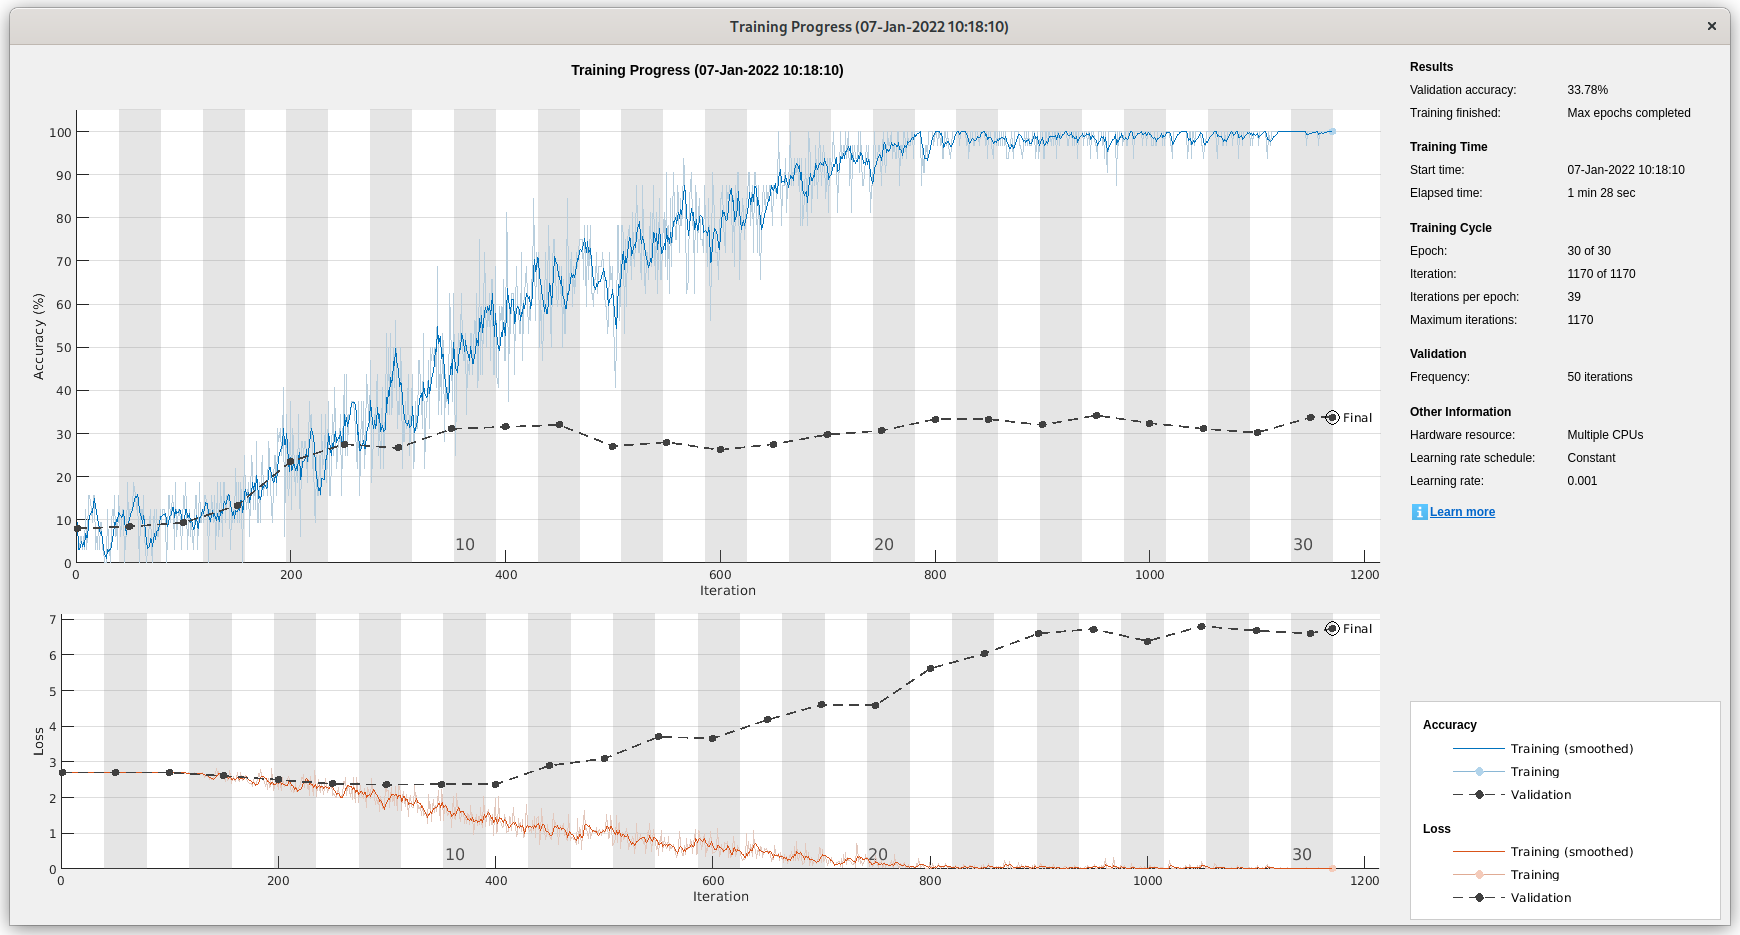
\includegraphics[ width=1.0\linewidth, height=\textheight, keepaspectratio]{./pics/maxepoch-overfitting.png}
        \caption{Overfitting of the network when \texttt{MaxEpoch} is the default value of $30$.}
        \label{fig:maxepoch-overfitting}
\end{figure}

With the goal of avoiding overfitting, a lower \texttt{MaxEpoch} value (for instance $8$) should be adopted.

\subsection{Fine-tuning initial learning rate}\label{sec:baseline-parameters}

Fine-tune the initial learning rate required manual trials along with manual inspection. Values of $0.1$, $0.01$, $0.001$ and $0.0001$ (representatives of various order of magnitude) were tried. Only values in the neighborhood of $0.001$ gave the required performance of around $30\%$. Since the default \texttt{MaxEpoch} value of $30$ led to overfitting, a lower number should be set.

In particular, testing the network $5$ times, with an optimal initial learning rate of $0.0005$, $0.001$, $0.0015$ and $8$ epochs, collecting the accuracy of each run and averaging the results returned the following Table~\ref{tab:baseline-accuracy},

\bigskip

\begin{table}[ht]
\centering
\begin{tabular}{|c|c|c|c|}
\hline 
\textbf{Initial learning rate} & \textbf{Average of validation accuracy} & \textbf{Average of test set accuracy} & \textbf{Epochs} \\
\hline \hline 
$0.0005$ & $0.2258$ & $0.1970$ & $8$ \\
\hline
$0.001$ & $0.2766$ & $0.2623$ & $8$ \\
\hline 
$0.0015$ & $0.2800$ & $0.2919$ & $8$ \\
\hline
\end{tabular}
\caption{Evaluating accuracy for different baseline networks.}\label{tab:baseline-accuracy}
\end{table}
\bigskip

Apparently, the baseline network of choice should be the third one with an initial learning rate of $0.0015$. However, the comparison is unfair since that network manifests signs of overfitting beginning with the Epoch $8$. To compare those two networks the group decided to lower the number of Epochs for the third network, and repeat the training:

\bigskip

\begin{table}[ht]
\centering
\begin{tabular}{|c|c|c|c|}
\hline 
\textbf{Initial learning rate} & \textbf{Average of validation accuracy} & \textbf{Average of test set accuracy} & \textbf{Epochs} \\
\hline \hline 
$0.001$ & $0.2766$ & $0.2623$ & $8$\\
\hline 
$0.0015$ & $0.2800$ & $0.2664$ & $7$\\
\hline
\end{tabular}
\caption{Evaluating accuracy for different baseline networks, with no overfitting.}\label{tab:baseline-accuracy-no-overfitting}
\end{table}
\bigskip

where in this case the choice makes no real difference with respect to the average of test set accuracy. To keep the baseline as simple as possible, the students decided to elect the first network as the \emph{baseline}, with parameters as in following Table~\ref{tab:baseline-parameters}:

\bigskip
\begin{table}[ht]
\centering
\begin{tabular}{|c|c|}
\hline 
\textbf{Parameter} & \textbf{Value} \\
\hline \hline 
Optimization Algorithm & sgdm \\
\hline 
Epochs (stopping criterion) & $8$\\
\hline 
Initial Learning Rate & $0.001$\\
\hline
MiniBatch size & $32$ \\
\hline
Weights initialization & Gaussian with $\mu = 0$ and $\sigma = 0.01$\\
\hline 
Bias initialization & $0$\\
\hline
\end{tabular}
\caption{Baseline parameters.}\label{tab:baseline-parameters}
\end{table}
\bigskip

\subsection{Baseline training progress and confusion matrix}

The overall training progress for the baseline network is shown in Figure~\ref{fig:baseline-progress}.

\begin{figure}[ht]
        \centering
        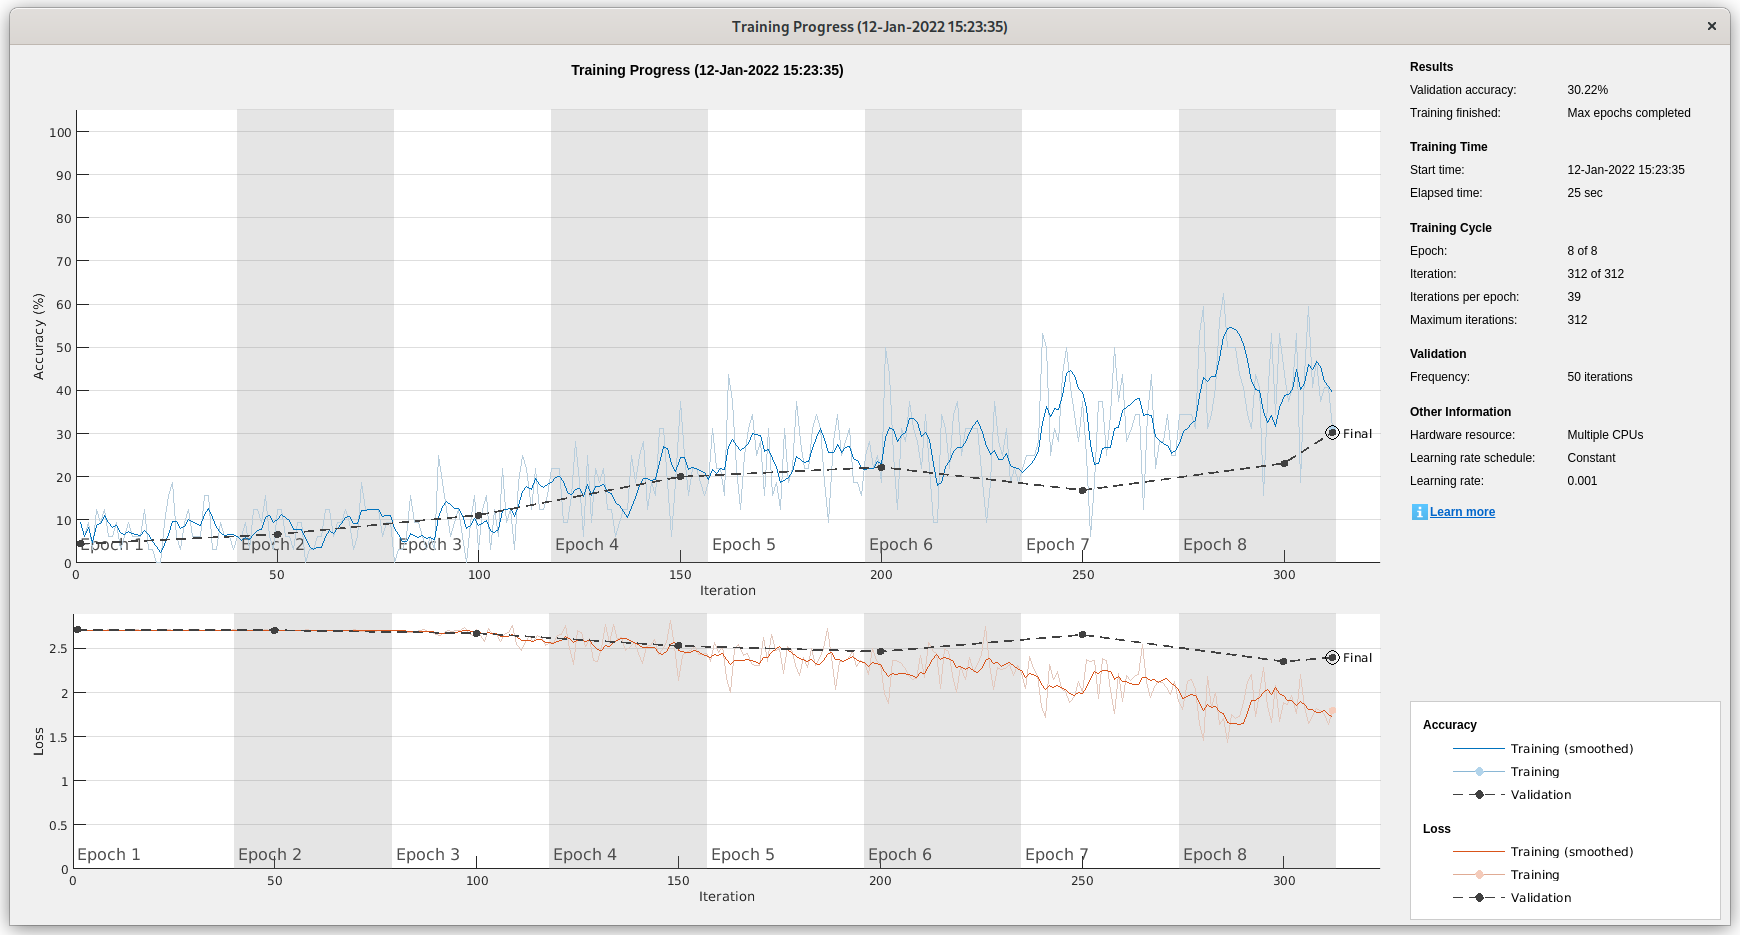
\includegraphics[ width=1.0\linewidth, height=\textheight, keepaspectratio]{./pics/baseline-progress.png}
        \caption{Training progress for the baseline network.}
        \label{fig:baseline-progress}
\end{figure}

To obtain the \emph{confusion matrix} for the chosen baseline network, the students ran the following code to first train the network again, and then plot a confusion matrix as shown in Figure~\ref{fig:baseline-confusion},

\begin{lstlisting}
InitialLearningRate = 0.001;
options = trainingOptions('sgdm', ...
    'InitialLearnRate', InitialLearningRate, ...
    'ValidationData',imdsValidation, ... 
    'MiniBatchSize',32, ...
    'MaxEpochs', 8,...
    'ExecutionEnvironment','parallel',...
    'Plots','training-progress'...
);

net = trainNetwork(imdsTrain,layers,options);

TestDatasetPath = fullfile('dataset','test');
imdsTest = imageDatastore(TestDatasetPath, ...
    'IncludeSubfolders',true,'LabelSource','foldernames');
imdsTest.ReadFcn = @(x)imresize(imread(x),[64 64]);

YPredicted = classify(net,imdsTest);
YTest = imdsTest.Labels;

accuracy = sum(YPredicted == YTest)/numel(YTest);

figure
plotconfusion(YTest,YPredicted)
\end{lstlisting}

\begin{figure}[ht]
        \centering
        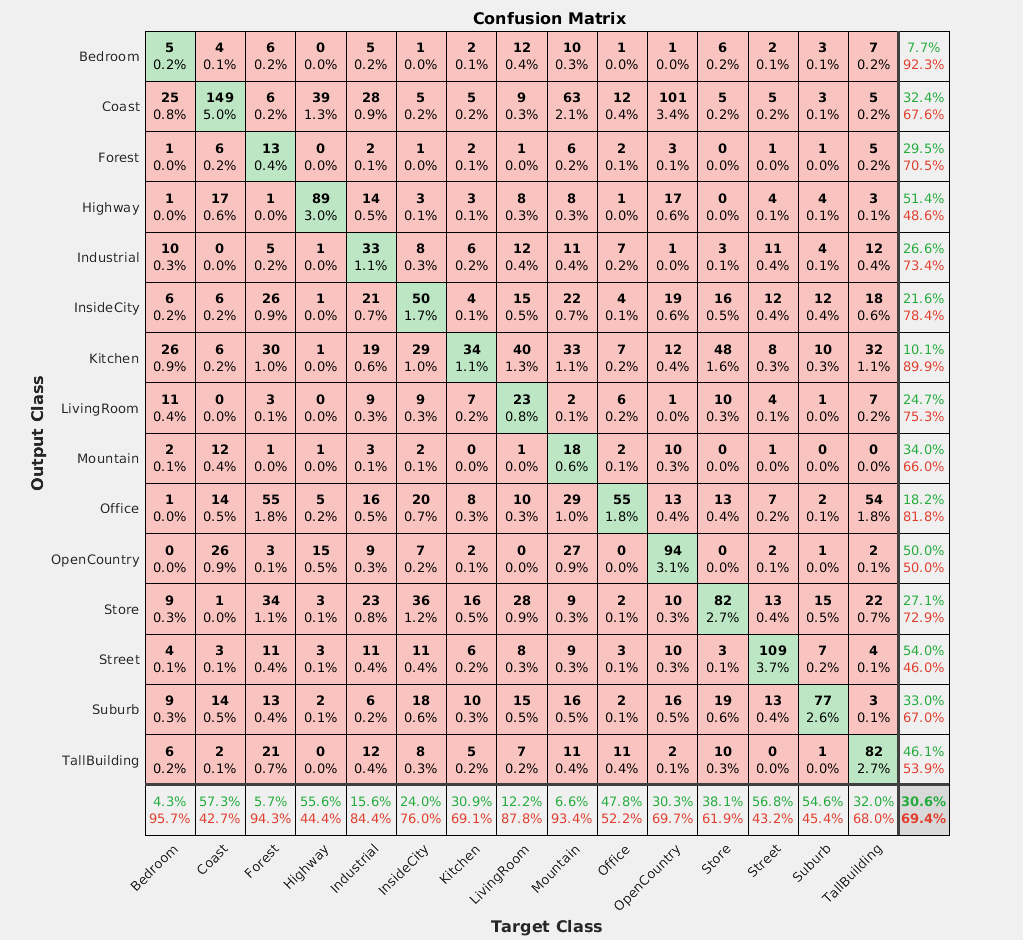
\includegraphics[ width=1.0\linewidth, height=\textheight, keepaspectratio]{./pics/baseline-confusion.png}
        \caption{Confusion matrix for the baseline network.}
        \label{fig:baseline-confusion}
\end{figure}

The confusion matrix shows that there are some classes that are more often misclassified (\texttt{kitchen}, \texttt{industrial}) and some classes that instead are less often misclassified, such as \texttt{highway} and \texttt{street}. Overall accuracy stands at the value $28.9\%$: from this point of view, the baseline should represent an improvement from a completely random classifier, whose performance with respect to this classification task is less than~a~$7\%$.

\clearpage

\section{Improving the network}\label{sec:improved-network}

The students propose (and have implemented) various methods in order to double the performance of the Convolutional Neural Network from the baseline $\sim 30\%$ to a $60\%$:

\begin{enumerate}
    \item \emph{data augmentation};
    \item addition of \emph{batch normalization layers};
    \item changing the \emph{size of the convolutional filters};
    \item modifying network layout;
\end{enumerate}

Individual contribution and net improvement of each of these methods is not investigated \--- what is provided, instead, is a description of each technique's implementation along with the necessary details, a brief description of the increasing improvements \emph{at each added complexity} and a final overview of all improvements altogether with respect to the baseline. 

\subsection{Data augmentation}\label{sec:data-augmentation}

The first improvement of the network is related to \emph{data augmentation}. The students implemented \emph{left-to-right reflections} of the train set, leaving unalterated the test set required for evaluation.

Running code 

\begin{lstlisting}
aug = imageDataAugmenter("RandXReflection",true);
imageSize = [64 64 1];
auimds = augmentedImageDatastore(imageSize,imdsTrain,'DataAugmentation',aug);
aunet = trainNetwork(auimds,layers,options);
\end{lstlisting}

with the same options as the baseline, but \texttt{MaxEpoch} set to $15$ (this kind of training resulted somehow to be slower), returned a validation accuracy of around $\sim 39\%$. Hence, the added complexity represented a slight improvement from the previous step.

\subsection{Batch normalization}

The second improvement should consist in adding $3$ \textbf{Batch Normalization layers} before the ReLU layers. Each layer should be added into \texttt{layers} object, by adding line

\begin{lstlisting}
batchNormalizationLayer('Name','BN_1')
\end{lstlisting} 

before any ReLU layer. The name of the new layers should be changed accordingly to the position of those layers.

The added complexity resulted in a faster learning (a lower MaxEpoch number should be set, from $15$ to $6$) and a much higher accuracy ($51.11\%$ on validation set, $48.7\%$ on test data).

\subsection{Improving convolutional layers}

Convolution layers may be improved by increasing the size of the filter as they are placed towards the output. In practice, this means modifying the convolution layers such that their size increases from $3\times 3$ only, to $3 \times 3$, $5\times 5$ and $7 \times 7$:

\begin{lstlisting}
convolution2dLayer(3,8,'Padding','same','Stride', [1 1], 'Name','conv_1',...
    'WeightsInitializer', @(sz) randn(sz)*0.01,...
    'BiasInitializer', @(sz) zeros(sz))

[...]

convolution2dLayer(5,16,'Padding','same','Stride', [1 1], 'Name','conv_2',...
    'WeightsInitializer',@(sz) randn(sz)*0.01,...
    'BiasInitializer', @(sz) zeros(sz))

[...]

 convolution2dLayer(7,32,'Padding','same','Stride', [1 1], 'Name','conv_3',...
    'WeightsInitializer', @(sz) randn(sz)*0.01,...
    'BiasInitializer', @(sz) zeros(sz))
\end{lstlisting}

This third addition brought a slight improvement, as the validation accuracy is at $55.11\%$, but the overall test accuracy stands at $50\%$.

\subsection{Modifying network layout}

Editing the layout of the network should improve the overall accuracy.

Since layout of the network changed, \emph{MaxEpoch} should be set accordingly, with the goal of avoiding overfitting while leaving the network room for enough complexity.

\subsubsection{Adding fully-connected and dropout layers}

A new fully-connected layer, along with a ReLU layer, were added:

\begin{lstlisting}
fullyConnectedLayer(256,'Name','fc_1',...
    'WeightsInitializer', @(sz) randn(sz)*0.01,...
    'BiasInitializer', @(sz) zeros(sz))
reluLayer('Name','relu_4')
\end{lstlisting}

A dropout layer separating the two fully-connected layers was added too,

\begin{lstlisting}
dropoutLayer(.25, 'Name', 'dropout_1')
\end{lstlisting}

\subsubsection{MaxEpoch}

In order to let the network have enough room for complexity, a \texttt{MaxEpoch} value of $25$ should be set.

\subsubsection{Results}\label{sec:results}

Overall network layout is illustrated in the following Table~\ref{tab:improved-network-layout}:

\begin{table}[ht]
\centering
\begin{tabular}{|c|c|c|}
\hline 
\textbf{\#} & \textbf{Layer type} & \textbf{Size and parameters} \\
\hline \hline 
1 & Image input & $64 \times 64 \times 1$ images \\
\hline 
2 & Convolution & $8 \mbox{ } 3 \times 3$ convolutions, stride 1 \\
\hline 
3 & Batch Normalization & \\
\hline
4 & ReLU &  \\
\hline 
5 & Max Pooling & $2 \times 2$ max pooling, stride 2 \\
\hline
6 & Convolution & $16 \mbox{ } 5 \times 5$ convolutions, stride 1 \\
\hline 
7 & Batch Normalization & \\
\hline
8 & ReLU &  \\
\hline 
9 & Max Pooling & $2 \times 2$ max pooling, stride 2 \\
\hline
10 & Convolution & $32 \mbox{ } 7 \times 7$ convolutions, stride 1 \\
\hline 
11 & Batch Normalization & \\
\hline
12 & ReLU & \\
\hline 
13 & Max Pooling & $2 \times 2$ max pooling, stride 2 \\
\hline
14 & Fully Connected & $256$ \\
\hline
15 & ReLU & \\
\hline
16 & Dropout & $25\%$ \\
\hline
17 & Fully Connected & $15$ \\
\hline
18 & Softmax & softmax \\
\hline
19 & Classification & crossentropyex \\
\hline
\end{tabular}
\caption{Improved Network layout.}\label{tab:improved-network-layout}
\end{table}
\bigskip

while training options are listed in the table below,

\bigskip
\begin{table}[ht]
\centering
\begin{tabular}{|c|c|}
\hline 
\textbf{Parameter} & \textbf{Value} \\
\hline \hline 
Optimization Algorithm & sgdm \\
\hline 
Epochs (stopping criterion) & $25$\\
\hline 
Initial Learning Rate & $0.001$\\
\hline
MiniBatch size & $32$ \\
\hline
Weights initialization & Gaussian with $\mu = 0$ and $\sigma = 0.01$\\
\hline 
Bias initialization & $0$\\
\hline
\end{tabular}
\caption{Improved Network parameters.}\label{tab:improved-network-parameters}
\end{table}
\bigskip


Students reported that these further improvements led to a \emph{validation accuracy} of around $60\%$, while the \emph{test accuracy} stands at a $57\%$ on average.

Training progress and confusion matrix, along with a comparison with the baseline, will be discussed in Section~\ref{sec:baseline-comparison}.

\subsection{Parameters and layout enhancements that did not provide benefit}\label{sec:no-benefits}

Students chose the simplest network among many others that did not bring much of an improvement. The choice of the simplest network has been determined by three factors:

\begin{enumerate}
    \item the network should have a higher overall accuracy when compared to others;
    \item if not, the network should not see its complexity increased with no tangible benefit performance-wise;
    \item if not, the network should be as much comparable as possible to the baseline (it should share the same parameters as much as possible).
\end{enumerate}

With this two fundamental goals in mind, the students discarded other configurations which did not result in significant improvements performance-wise, or introduced higher complexity, with less parameters shared between the improved network and the baseline.

In particular,

\begin{itemize}
    \item increasing or lowering the size of \emph{MiniBatch} has not been sufficient to improve performance \--- however, it changed significantly the behavior of the training phase, which required setting the \emph{initial learning rate} to a different value;
    \item switching the optimization algorithm to \emph{adam} has not been sufficient to show significant improvements, even after fine-tuning parameters. Students tried many different variants of the network with the adam optimization algorithm, however the results were not good enough to justify the switch;
    \item adding any convolutional layer did not result in performance improvements.
\end{itemize}


\subsection{Comparison with the baseline}\label{sec:baseline-comparison}

The students collected pictures of training progress and relative confusion matrix of both \emph{baseline network} (parameters in Section~\ref{sec:baseline-parameters}) and \emph{improved network} (parameters in Section~\ref{sec:results}).

Figure~\ref{fig:comparison-confusion} shows that classes that had been better predicted by the baseline network are still among those better predicted by the improved network too (for instance, \emph{Street} and \emph{TallBuilding}), while some other classes that were initially difficult have seen a huge improvement (\emph{Bedroom}, \emph{Forest}, \emph{Kitchen}).

In general, the improved network shows significant better performance when compared to the baseline network (an almost doubled accuracy on both validation and test set), at the cost of added complexity and some more training time required. Other variants of the improved network were tried by varying parameters and layout as described in Section~\ref{sec:no-benefits}, but no significant accuracy improvements justified the applied changes.

\begin{figure}[ht]
        \centering
        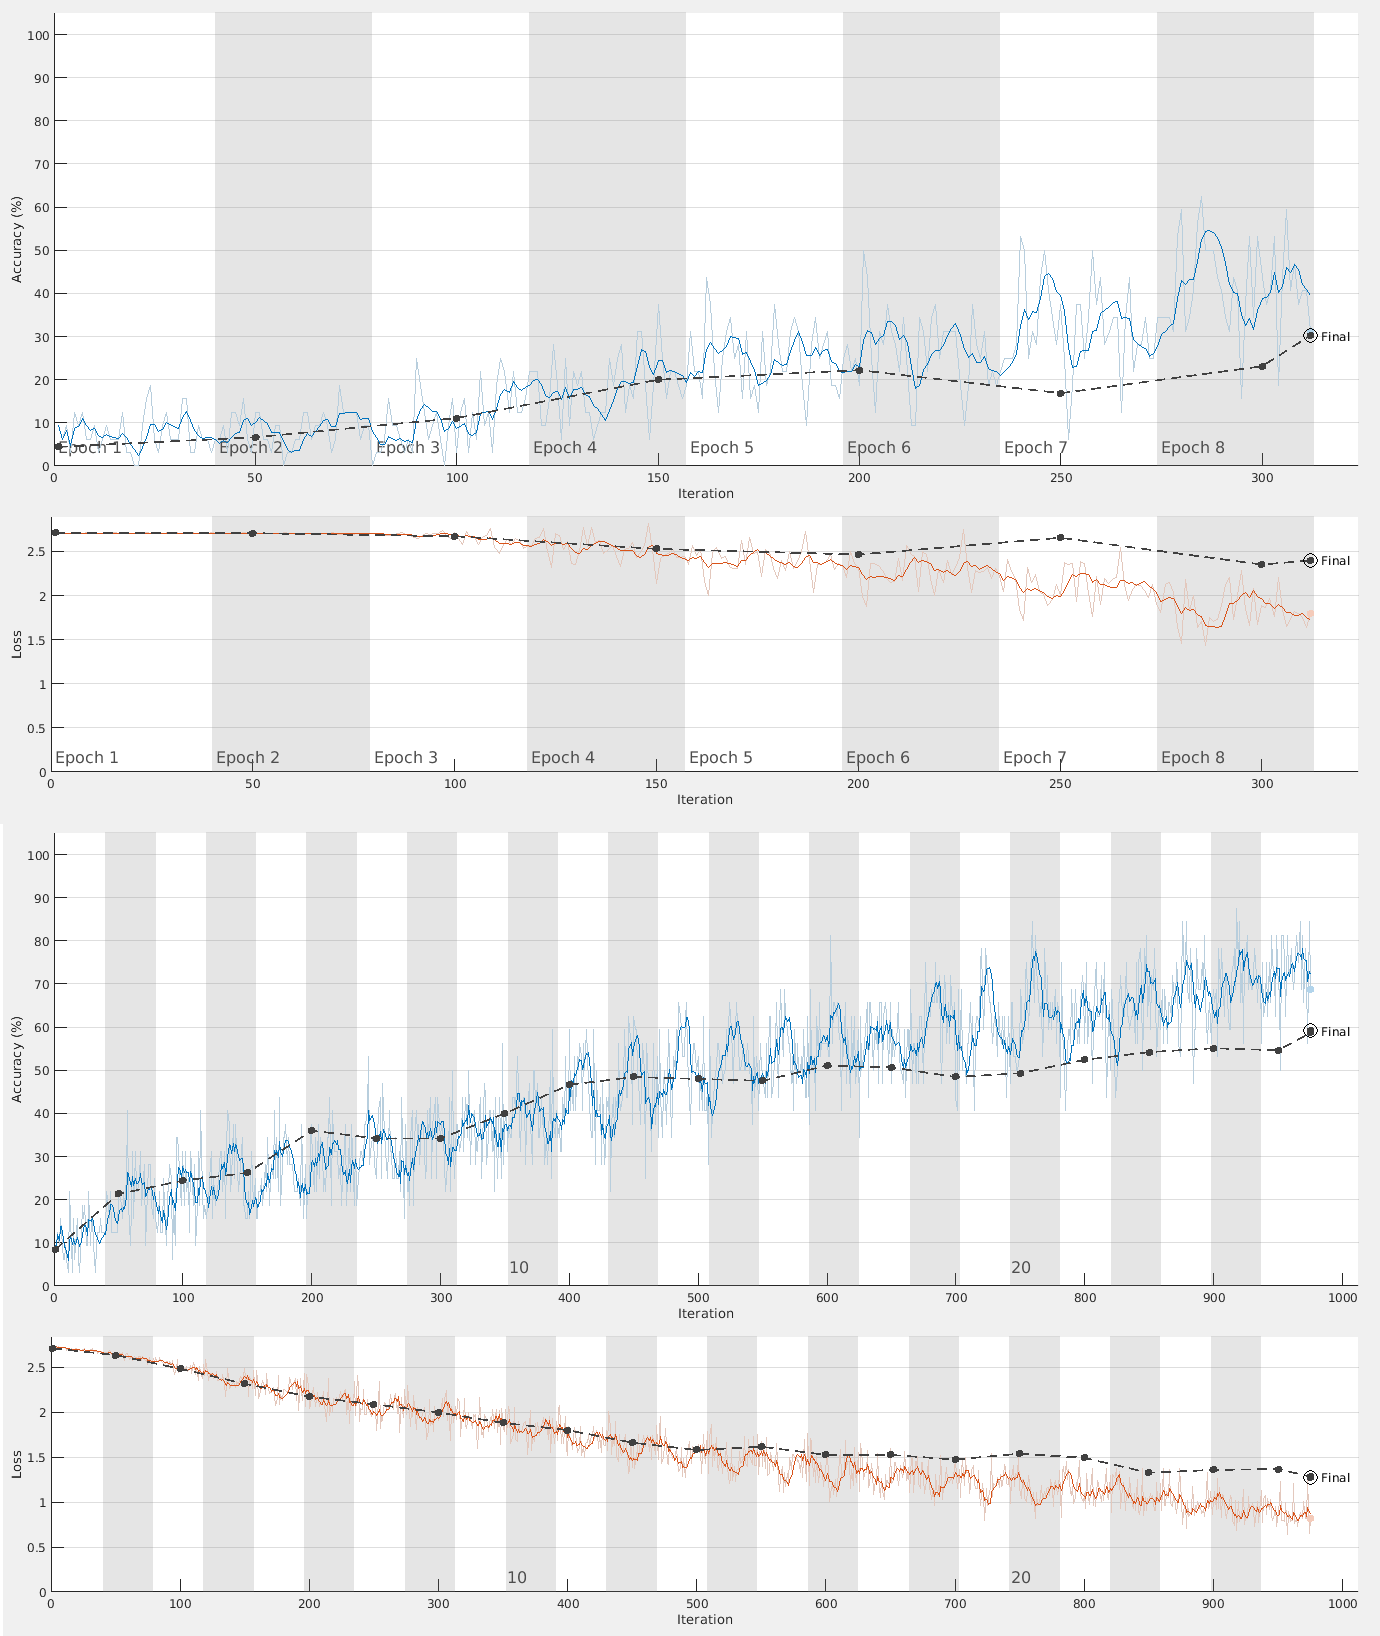
\includegraphics[ width=1.0\linewidth, height=\textheight, keepaspectratio]{./pics/comparison-progress.png}
        \caption{Comparison between training progress of the baseline network (on top) and training progress of the improved network (on bottom).}
        \label{fig:comparison-progress}
\end{figure}

\begin{figure}[ht]
        \centering
        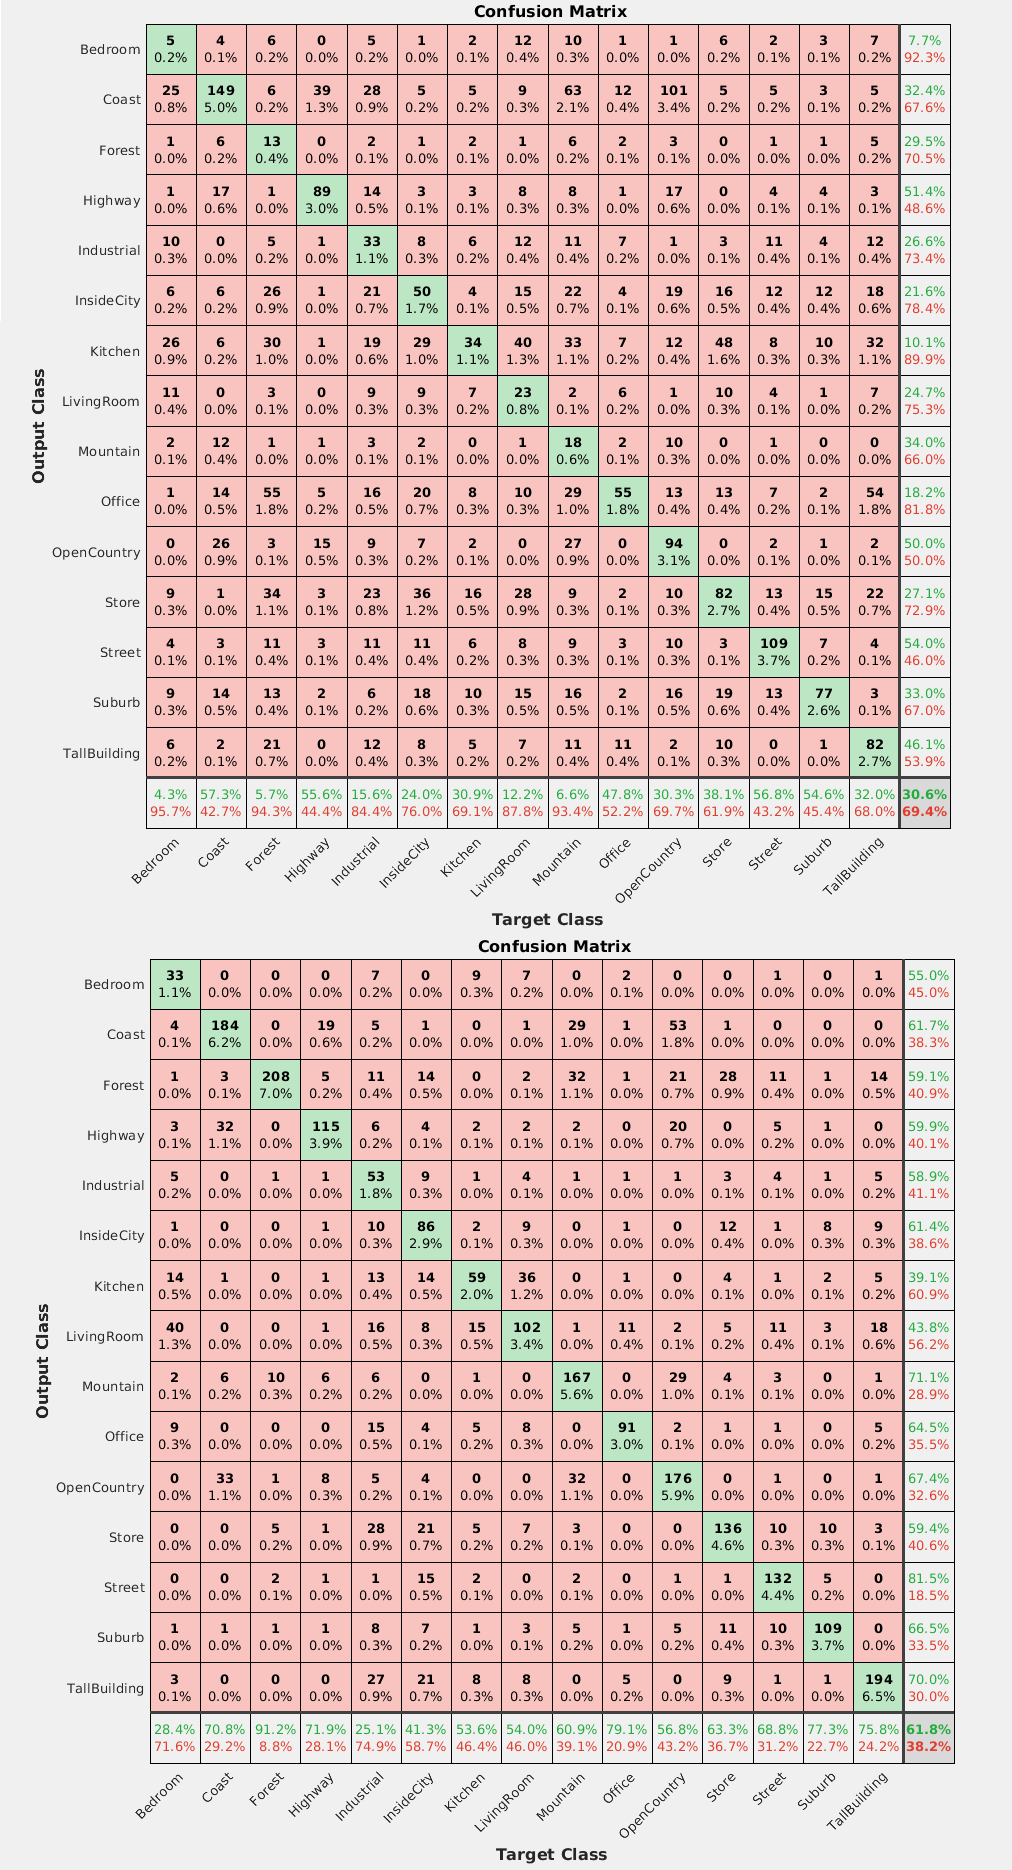
\includegraphics[ width=0.8\linewidth, height=0.8\textheight, keepaspectratio]{./pics/comparison-confusion.png}
        \caption{Comparison between confusion matrices of the baseline network (top) and the improved network (bottom).}
        \label{fig:comparison-confusion}
\end{figure}

\clearpage

\subsection{Ensemble network based on previous improvements}

The students implemented an \textbf{ensemble network}, composed of $5$ networks of the same layout as in Section~\ref{sec:results}. In order to assign the class, a \emph{voting} system has been built: each network of the ensemble casts a vote (a class), and the overall output is the \emph{most common predicted class} among the ensemble.

The code related to the ensemble prediction is the following one,

\begin{lstlisting}
% Evaluating ensemble network accuracy

EnsembleNum=5;
for i=1:EnsembleNum
    YPred = classify(net(i),imdsTest);
    for j=1:size(YPred)
        YPredicted(j,i) = YPred(j);
    end
end    

categ = categorical(categories(YTest));
for i=1:size(YPred)
    [v, argmax] = max(countcats(YPredicted(i,:)));
    predicted_output(i) = categ(argmax);
end

accuracy = sum(predicted_output == YTest)/numel(YTest);
figure
plotconfusion(YTest, predicted_output')
\end{lstlisting}

where \texttt{net(i)} is a network belonging to an array of $5$ trained networks. As a result, the above code will plot a confusion matrix for the ensemble network.

\subsection{Justifying the added complexity}

Ensemble training is very heavy on resources. Time training multiple networks is significantly higher than the time required for training a single network, let alone the time necessary for both training and classifying with an ensemble of networks. Hence, the students questioned themselves whether an ensemble of more networks (for instance, $10$ networks or more) could bring any improvement with respect to an ensemble of $5$ or less.

In order to answer the question, the students collected test accuracy of ensemble networks of different number $B$ of networks, and compared them with the average of every single network in the ensemble. Each ensemble network has been trained separately, and results has been collected in the following Table~\ref{tab:ensemble-evaluation},

\begin{table}[ht]
\centering
\begin{tabular}{|c||c|c|c|}
\hline
\textbf{B} & \textbf{Single networks average accuracy} & \textbf{Ensemble test set accuracy} & \textbf{Net improvement}\\
\hline
\hline
3 & $0.5763$ & $0.5950$ & $1.87\%$ \\
\hline
5 & $0.5863$ & $0.6280$ & $4.17\%$ \\
\hline
7 & $0.5868$ & $0.6340$ & $4.72\%$\\
\hline
10 & $0.5841$ & $0.6410$ & $5.69\%$\\
\hline
15 & $0.5871$ & $0.6470$ & $5.99\%$\\
\hline
\end{tabular}
\caption{Ensemble network accuracy evaluation.}\label{tab:ensemble-evaluation}
\end{table}

Basically, training an ensemble of $B=5$ networks should be enough to provide tangible benefits, with even higher improvements over the single networks when training a $B=10$ ensemble network (although the improvements are not so pronounced).

Training the network with $B=15$ only introduced a moderate improvement, thus such a high number of networks is not strictly required and would instead offer more disadvantages than advantages (for instance, training and classification time) with respect to an ensemble network having only $5$ or $10$ networks.

At every run, ensemble networks had shown more accuracy on the test set with respect to the single network. In addition, the single network performance is very unreliable, largely depending on the randomness of the learning phase, with test set accuracy values ranging from $55\%$ to over $60\%$ \--- on contrary, the ensemble network accuracy has proven to be much more reliable over different runs. On this particular task, ensemble learning has proven to be effective \--- however, its increased complexity and time required for training and classification cannot be undervalued. A good trade-off between net~improvement and increased complexity could be a choice of $B=5$ networks for the ensemble network, which should bring the accuracy of the student's proposed model well-above $60\%$.
 
\section{Adopting transfer learning with AlexNet}
\subsection{Transfer learning by freezing weights}

In the third section, the students were required to adopt transfer learning based on a pre-trained network. The network of choice has beed \emph{AlexNet}: the first $22$ layers of the network have been preserved, while only the last $3$ were replaced by the last $3$ layers of the improved network. Moreover, since the goal of transfer learning should be to adopt a pre-trained network with no further learning of its layers, the weights of the AlexNet layers have been freezed, preventing them to be modified during the learning phase. 

The layout of the transfer learning network is described in Table~\ref{tab:transfer-learning-layout-1}:

\bigskip
\begin{table}[ht]
\centering
\begin{tabular}{|c|c|c|}
\hline 
\textbf{\#} & \textbf{Layer type} & \textbf{Size and parameters} \\
\hline \hline 
$1:22$ & AlexNet layers & weights freezed \\
\hline 
$23$ & Fully Connected & $15$ \\
\hline
$24$ & Softmax & softmax \\ 
\hline 
$25$ & Classification & crossentropyex \\
\hline
\end{tabular}
\caption{Transfer Learning Layout}\label{tab:transfer-learning-layout-1}
\end{table}
\bigskip

The code that produced the specified layout is the following one,

\begin{lstlisting}
net = alexnet;

layersAlex = net.Layers(1:end-3);

layers = [
    layersAlex

    fullyConnectedLayer(15,'Name','fc_2',...
        'WeightsInitializer', @(sz) randn(sz)*0.01,...
        'BiasInitializer', @(sz) zeros(sz))

    softmaxLayer('Name','softmax')
    classificationLayer('Name','output')
];

layers(1:end-3) = freezeWeights(layers(1:end-3));
\end{lstlisting}

where the function \texttt{freezeWeights} has been obtained as-is from an online git repository (\href{https://github.com/GRSEB9S/Transfer-Learning-using-Matlab/blob/master/TransferLearningUsingResNet101Example/freezeWeights.m}{URL}), and will be reported here:

\begin{lstlisting}
function layers = freezeWeights(layers)
% layers = freezeWeights(layers) sets the learning rates of all the
% parameters of the layers in the layer array |layers| to zero.

for ii = 1:size(layers,1)
    props = properties(layers(ii));
    for p = 1:numel(props)
        propName = props{p};
        if ~isempty(regexp(propName, 'LearnRateFactor$', 'once'))
            layers(ii).(propName) = 0;
        end
    end
end

end
\end{lstlisting}

\subsubsection{Input layer}

The students adopted the same data augmentation techniques that has been shown in Section~\ref{sec:data-augmentation}. In order to preserve the input layer of the AlexNet (along with its subsequent structure), an input size of $227 \times 227 \times 3$ should be guaranteed. To get the correct input size students had to first modify the picture size accordingly, and then to implement a greyscale to RGB conversion. The group adopted the simple approach to replicate the greyscale image $3$ times, creating the $3$ color channels by simply providing the greyscale information to each channel.

The code relative to this part is the following one,

\begin{lstlisting}
imds = imageDatastore(TrainDatasetPath, ...
    'IncludeSubfolders',true,'LabelSource','foldernames');
imds.ReadFcn = @(x)imresize(cat(3, imread(x), imread(x), imread(x)), [227 227]);
trainQuota=0.85;
[imdsTrain,imdsValidation] = splitEachLabel(imds,trainQuota,'randomize');
aug = imageDataAugmenter("RandXReflection",true);
imageSize = [227 227 3];
auimds = augmentedImageDatastore(imageSize,imdsTrain,'DataAugmentation',aug);
\end{lstlisting}

Notably, the main difference with respect to the previous sections is in the \texttt{ReadFcn} definition, where the image is first replicated into the $3$ RGB channels, then rescaled to the desired size.

\subsubsection{Training options}

Different training options were explored. The group found out that good training options could be the following ones,

\begin{lstlisting}
options = trainingOptions('sgdm', ...
    'MiniBatchSize',10, ...
    'MaxEpochs',6, ...
    'InitialLearnRate',1e-4, ...
    'ValidationData',imdsValidation, ...
    'ValidationFrequency',3, ...
    'Verbose',false, ...
    'Plots','training-progress');
\end{lstlisting}

\subsubsection{Results}

The training of the network provided an accuracy of $84.44\%$ in the validation set, and of $86.4\%$ in the test set, bringing overall accuracy well-above the $60\%$ of the improved network illustrated in Section~\ref{sec:improved-network}. Corresponding training progress and confusion matrix are provided in Figure~\ref{fig:transfer-learning-progress-1} and Figure~\ref{fig:transfer-learning-confusion-1}.


\begin{figure}[ht]
        \centering
        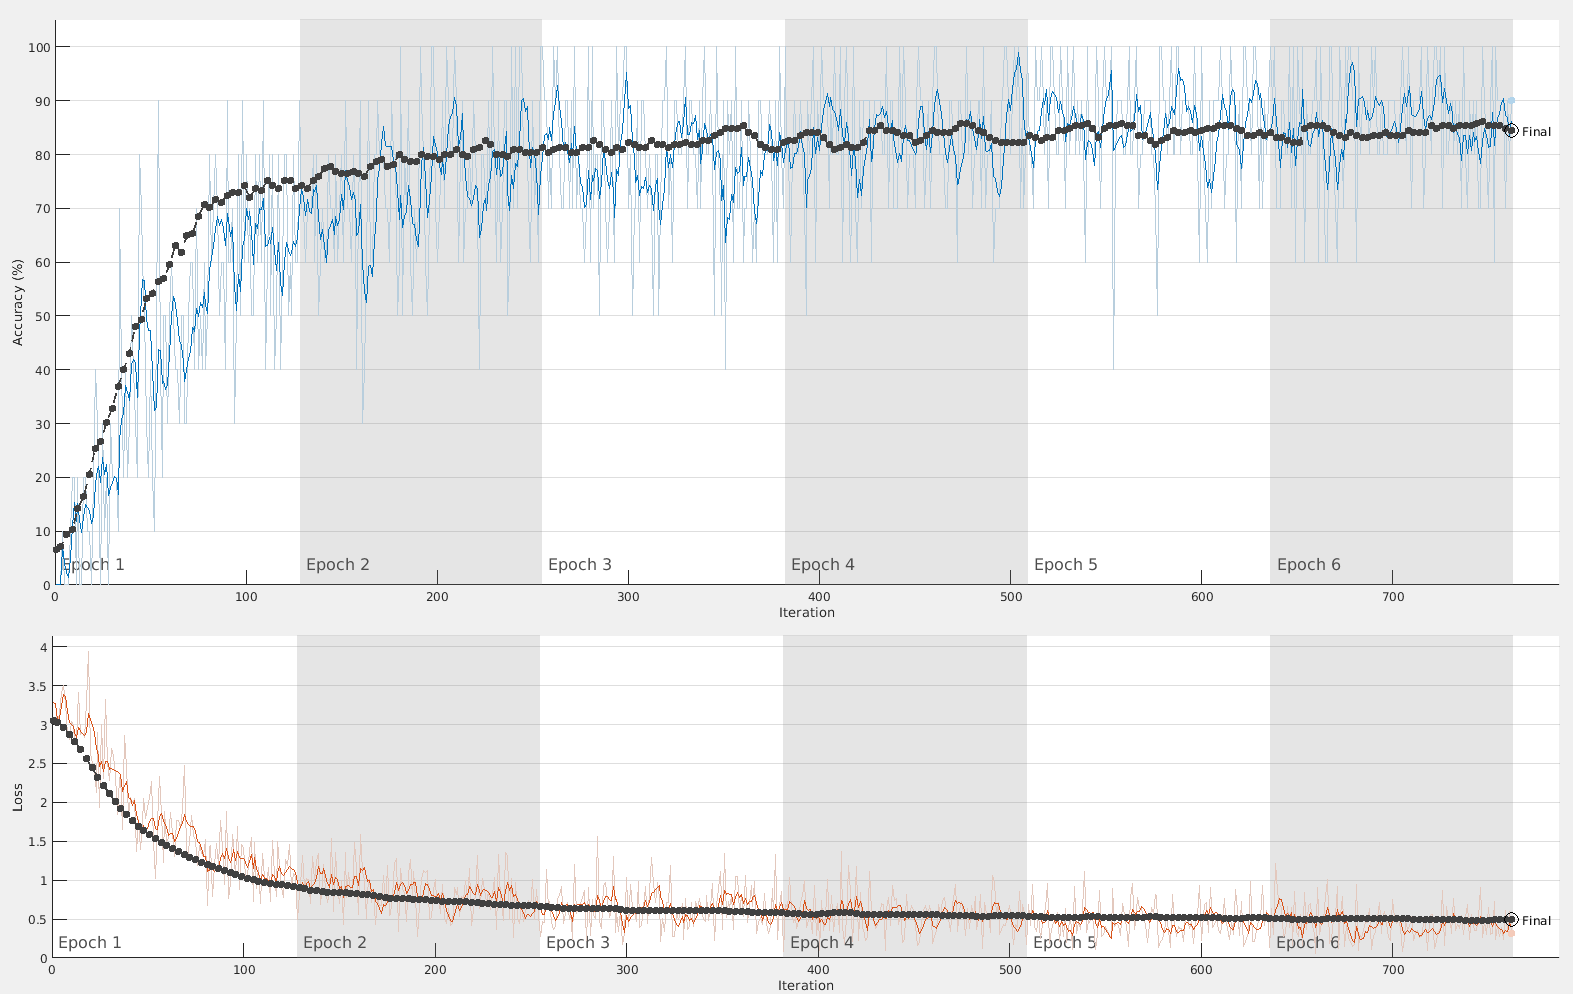
\includegraphics[ width=1.0\linewidth, height=\textheight, keepaspectratio]{./pics/transfer-learning-progress-1.png}
        \caption{Progress of the transfer learning network, employing AlexNet.}
        \label{fig:transfer-learning-progress-1}
\end{figure}


\begin{figure}[ht]
        \centering
        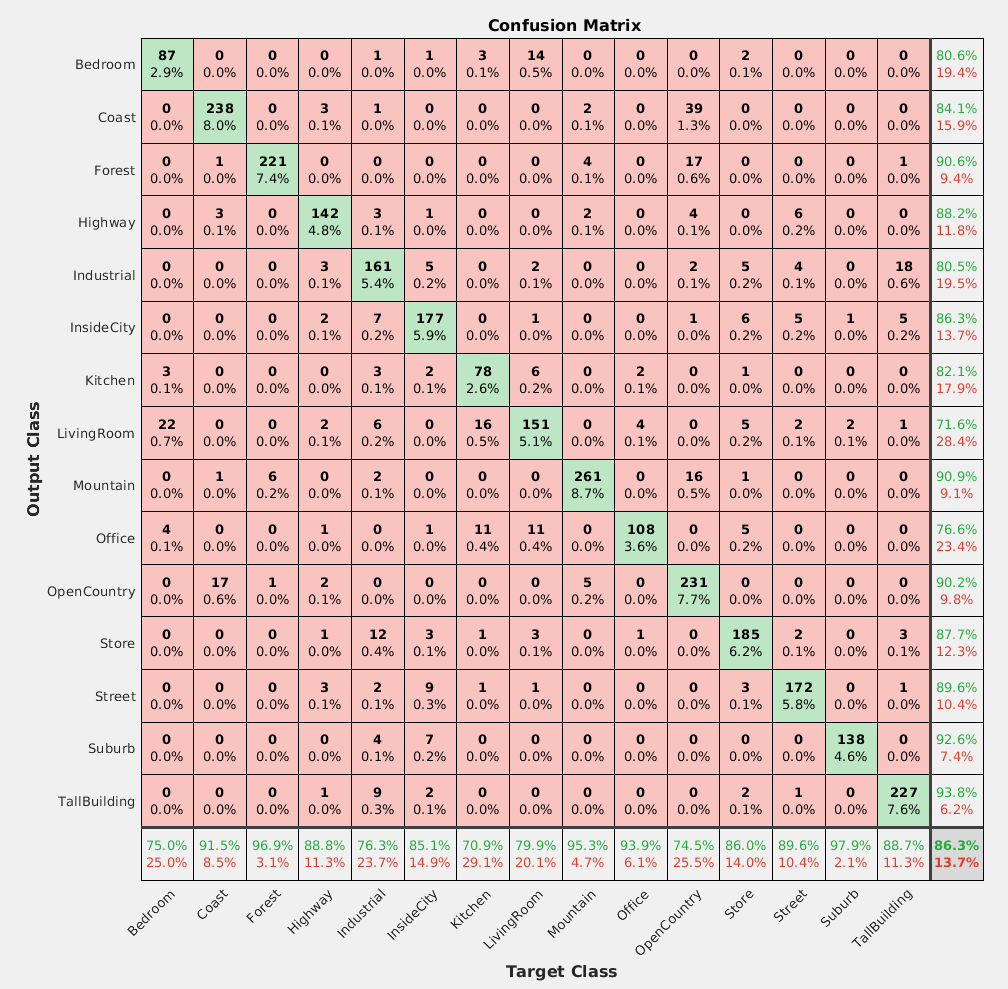
\includegraphics[ width=1.0\linewidth, height=\textheight, keepaspectratio]{./pics/transfer-learning-confusion-1.png}
        \caption{Confusion matrix of the transfer learning network.}
        \label{fig:transfer-learning-confusion-1}
\end{figure}

\clearpage




\subsection{AlexNet as feature extractor}

\end{document}
